\subsubsection{OBD II}
Die OBD-II Schnittstelle ist eine normierte, standardisierte Schnittstelle, welche, mittels einem passenden Auslesegerät, Zugriff auf die Daten den Motormanagements verschafft. Diese Schnittstelle hat unterschiedliche Versionen, welche auf die verschiedenen Kontinente aufgeschlüsselt wurden. Es gibt also OBD II, was Initial eine Schnittstelle der vereinigten Staaten war, weshalb der Standard auch in Nordamerika seit 1996 verbaut wurde. Zusätzlich gibt es EOBD, womit die europäische Umsetzung des OBD II Standards beschrieben wird.\cite{Directive.98/69/EC.EUParliament} Der wesentliche Unterschied ist dabei die Standardisierung, welche zwar technisch zwischen SAE J1962 und ISO/DIS 15031 gleich ist, aber trotzdem unterschiedlich benannt wurde. \cite{SAE.J1962} Ferner gab es eine australische \cite{AU.Motor.Vehicle.Standards.Act.1989} und eine japanische Version der Standardisierung.
\newline
\newline
Ausserdem gibt es eine, ebenfalls in der Standardisierung festgehalten einen OBD II A und B Konnektor. Der A Konnektor ist für alle Fahrzeuge mit 12 V Bordspannung und hat die Form eines D mit einer Nut in der Mitte, um die Pins zu behausen. Der B Konnektor verwendet ebenfalls die Form eines D's, allerdings ist dieser Konnektor für Fahrzeuge mit 24V Bordspannung, was häufig Lastkraftfahrzeuge sind. Bei diesem Konnektor ist die Nut in der Mitte unterbrochen, um es unmöglich zu machen einen männlichen Konnektor des A-Typs einzustecken. Dieser Konnektor könnte folglich nämlich aufgrund von Überspannung defekt werden. Es ist also der B Konnektor sowohl mit A und B kompatibel, allerdings ist der A Konnektor nur mit seinesgleichen verwendbar.


\begin{figure}[!htb]\centering
   \begin{minipage}{0.49\textwidth}
     \frame{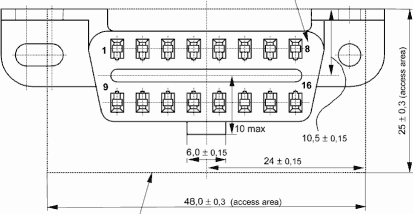
\includegraphics[width=\linewidth]{images/j1962f_type_a}}
     \caption{Typ A, OBD II Konnektor \cite{OBDII.TypeA}}\label{Fig:Data1}
   \end{minipage}
   \begin {minipage}{0.49\textwidth}
     \frame{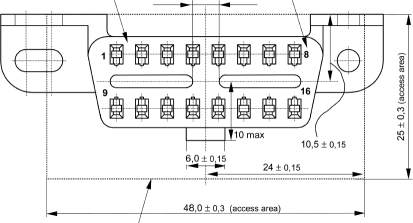
\includegraphics[width=\linewidth]{images/j1962f_type_b}}
     \caption{Typ B, OBD II Konnektor \cite{OBDII.TypeB}}\label{Fig:Data2}
   \end{minipage}
\end{figure}
